\chapter{Trabalhos relacionados}\label{cap:introducao}

Giovanni \citeonline[p.~117]{mori_analysing_2015} sugere que conceitos de práticas diversas, especialmente aqueles desenvolvidos no campo da Música, são agregados durante uma \emph{sessão} de \emph{live coding}: ``\emph{Live coding} é uma técnica artística de improvisação. Pode ser empregada em muitos contextos performativos diferentes: dança, música, imagens em movimento e mesmo tecelagem.'' \cite[p.~117]{mori_analysing_2015}\footnote{Tradução de \emph{Live coding is an improvisatory artistic technique. It can be employed in many different performative contexts: dance, music, moving images and even weaving. I have concentrated my attention on the music side, which seems to be the most prominent.}} (ver \autoref{fig:wavecoding}).

\begin{figure}[!h]
  \centering
  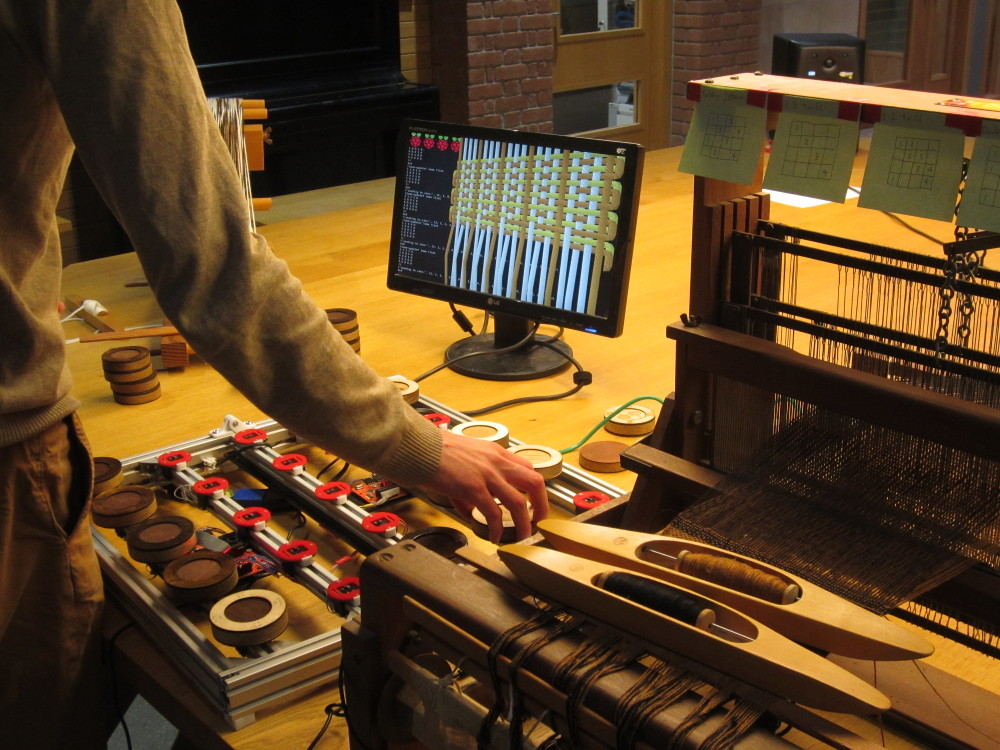
\includegraphics[scale=0.85]{imagens/wavecoding.jpg}
  \caption{Performance por Alex McLean,  David Griffiths, e \emph{Wavecoding group} (2015) utilizando uma máquina manual de tecelagem para realização de uma improvisação audiovisual em Falmouth, Cornwall (\url{http://fo.am/kernow/}) \textbf{Fonte}: \url{http://www.pawfal.org/dave/blog/category/slub/}.}
  \label{fig:wavecoding}
\end{figure}

Estas agregações dependem muito do contexto. Por exemplo, o \emph{live coding} pode ocorrer formalmente ou informalmente. Um exemplo da primeira situação é a performance \emph{screenBashing} (2015) de Magno Caliman (ver \autoref{fig:screenbashing}), realizada durante um concerto em Campinas-SP no ano de 2015. 

\begin{figure}[!h]
  \centering
  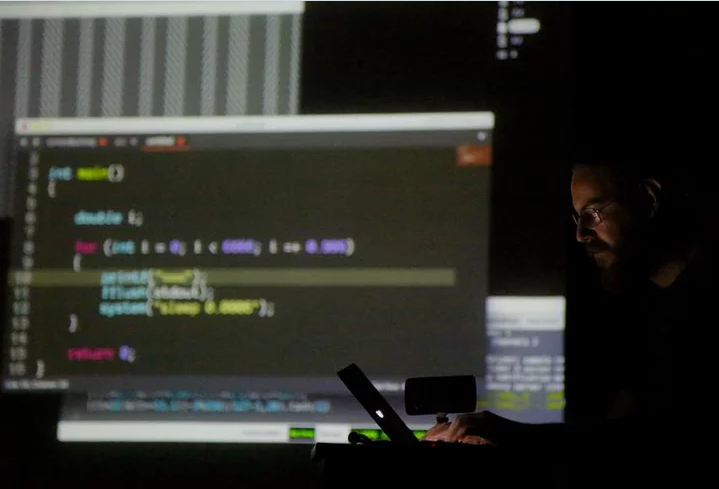
\includegraphics[scale=0.5]{imagens/screenbashing.png}
  \caption{Performance de \emph{screenBashing} durante o XIII ENCUN 2015 - Campinas (SP). A performance é um exemplo claro da estética \emph{noise} dentro do \emph{live coding}. Utiliza a linguagem C para gerar saídas textuais, utilizadas como texturas visuais, e o programa \emph{SuperCollider} para síntese sonora. \textbf{Fonte}: \url{https://vimeo.com/148626379}.}
  \label{fig:screenbashing}
\end{figure}

Informalidades incluem performances conhecidas como \emph{algoraves}. Apresentamos um exemplo do duo mexicano Mico Rex, em um circuito que percorreu as cidades de Brighton, Londres, Karlesruhe, Colonia e Dusseldorf (2013), evento permeado de música eletrônica de pista produzida pela programação de algoritmos (ver \autoref{fig:algorave}). \citeonline[p.~356]{collins_algorave:_2014} descreve o \emph{algorave} como uma atividade de \emph{code DJing}, ou um ``Disk Jockey codificado'':

\begin{citacao}
Executantes de \emph{algorave} apresentam um campo eclético de musicistas eletrônicos, usando predominantemente um laptop, mas também incluindo alguns experimentos no controle de hardware (\ldots) Por exemplo, \emph{sick lincoln} simultaneamente combinou DJ codificado no \emph{SuperCollider}, \emph{live coding} em um aplicativo \emph{Web Audio API}/\emph{javascript} e refabricação de \emph{patchs} de um sistema algorítmico no Max/MSP.\footnote{Tradução nossa de \emph{Algorave performers present an eclectic range of electronic musicians, predominantly using laptop alone, but also including some experiments in control of hardware (\ldots)  For example, \emph{sick lincoln} has simultaneously combined code DJing from SuperCollider, live coding from a Web Audio API javascript app and live repatching of a Max/MSP algorithmic hip hop system}. Sobre \emph{Web Audio API} e Javascript, ver \citeonline{roberts_gibber:_2012}. Javascript é uma linguagem de programação utilizada para realização de rotinas em páginas \emph{web}. Sobre Max/MSP, \url{}}
\end{citacao}

\begin{figure}[!h]
  \centering
  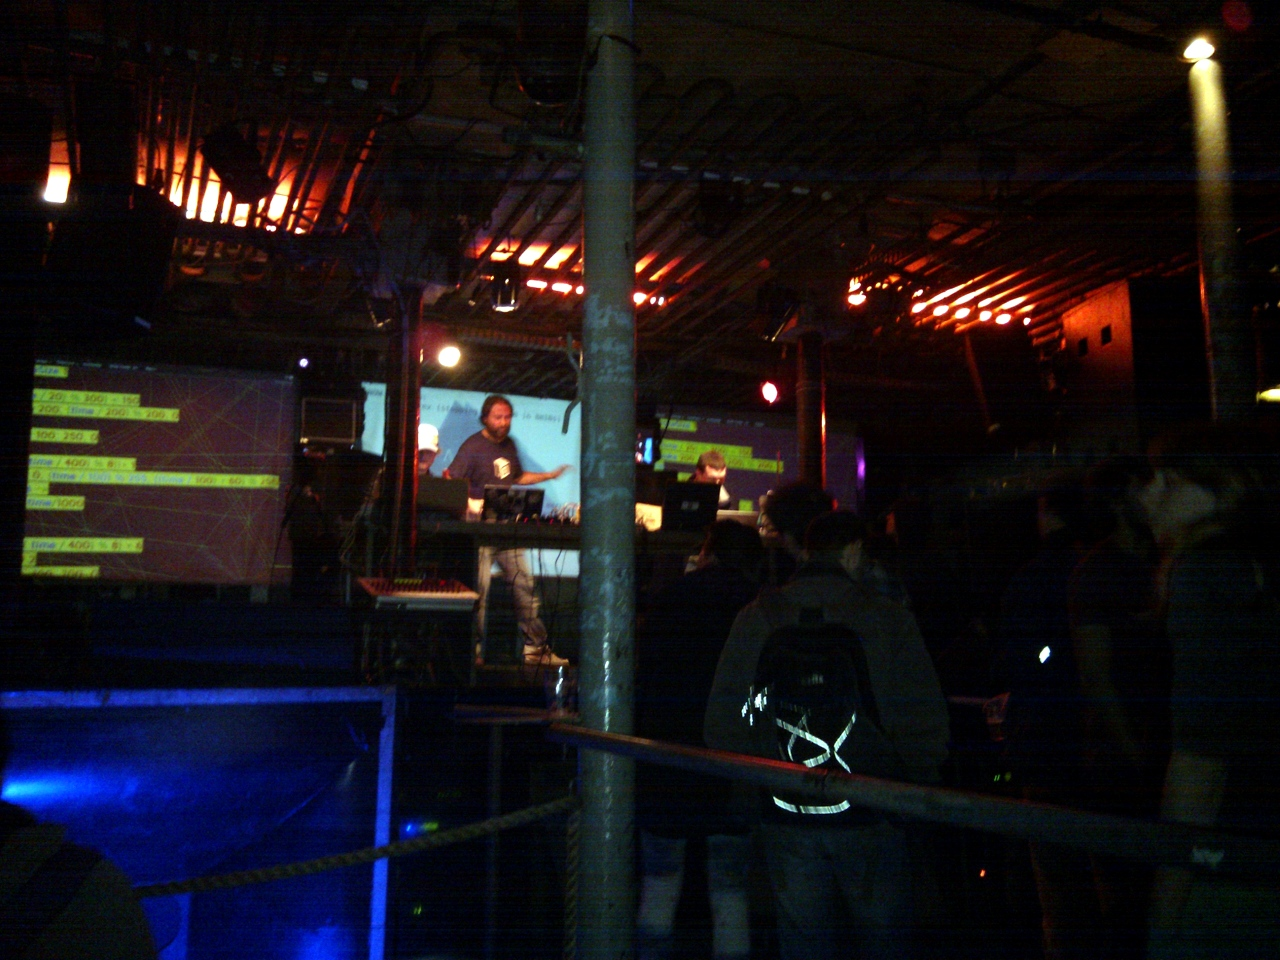
\includegraphics[scale=0.3]{imagens/algorave.jpg}
  \caption{Performance de Mico Rex durante o \emph{Algorave tour} (2013) \textbf{Fonte}: \url{http://www.pawfal.org/dave/blog/2013/04/life-on-an-algorave-tour/}.}
  \label{fig:algorave}
\end{figure}

O campo de atuação do \emph{live coding} é dinâmico, e depende de sua aplicação. Expomos três limites da prática, mas certamente existem outras abordagens. Enumerar todas pode ofuscar aquilo que queremos chamar a atenção: a multiplicidade de conceitos, seus limites e transições.

Uma primeira exposição desses diversos conceitos pode ser visualizada na \autoref{fig:nuvemlivecoding}; a figura foi feita com o auxílio de um programa descrito no \autoref{app:C}, e melhor explorada no \autoref{app:A}. 

\begin{figure}[!h]
\begin{center}
\centering
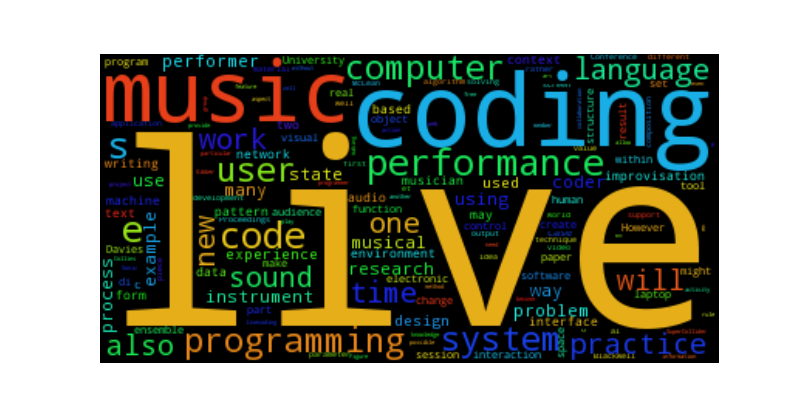
\includegraphics[scale=0.8]{./imagens/livecoding_cloud1.png}
\caption{Nuvem de palavras do \citeonline{ICLC2015},  1$^o$ Congresso Internacional de Live Coding. \textbf{Fonte}: autor.}
\label{fig:nuvemlivecoding}
\end{center}
\end{figure}


\section{Improvisação e Sistemas Criativos}\label{sec:universo}

Qualquer que seja a categorização dada ao \emph{live coding}, o termo \emph{live} transparece um assunto articulador: \emph{improvisação}. Definições do \emph{Universo de Conceitos para McLean}, e  o \emph{Modelo de Improvisação} de Pressing, serão discutidos na \autoref{cap:metodologia} como o método de investigação realizado.


\section{\emph{live coding}}\label{cap:trabalhos_relacionados}

Na \autoref{sec:groove}, descrevemos um trabalho de \citeonline{mathews_groove_1970}, GROOVE, ainda pouco observado por \emph{live coders}. Seu paradigma composicional é diverso do MUSIC N, e o primeiro de Mathews com reflexões nos aspectos performáticos. Não foi usado para ambientes de performance, mas a peça \emph{The expanding universe} da compositora Laurie \citeonline{spiegel_expanding_1975} foi considerada.

Na \autoref{sec:grossi}, \citeonline{mori_pietro_2015}  descreve um caso prematuro de \emph{live coding} na Itália, com o compositor Pietro Grossi (1917-2002).Divergente em algumas das propostas de Max Mathews, sacrificou a questão timbrística para trabalhar na questão performática.

Descrevemos, na seção \autoref{sec:baiasaofranscisco}, as atividades dos grupos \emph{The Hub} e \emph{The League of Automatic Composers} como fundamentais para o entendimento histórico do \emph{live coding}.

Sugerimos na \autoref{sec:jit} apontar a tecnologia JIT \cite{aycock_brief_2003} como um sujeito sócio-técnico fundamental para que o \emph{live coding} fosse possível.

Uma revisão de um trecho da publicação ``\emph{Live Algorithm Programming and Temporary Organization for its Promotion}'', de \citeauthoronline{mclean_patterns_2009}, será feita na \autoref{sec:laptoptoplap} para discutir identidade cultural da organização TOPLAP. 

Na \autoref{sec:showusyourscreens}, ``Show us your screens'', é revisto como o manifesto que define as regras heurísticas do \emph{live coding}.

\subsection{GROOVE}\label{sec:groove}

GROOVE, ou \emph{Generated Real-time Operations On Voltage-controlled Equipment} foi um computador desenvolvido na Bell Labs por \cite{mathews_groove_1970}. Alex \citeonline{di_nunzio_genesi_2010} discute como um precedente direto do MUSIC V, mas como um projeto bifurcado da família MUSIC N\footnote{Desenvolvidos a partir de 1957. \emph{softwares} MUSIC I, II, III, IV, IV-B, IV-BF, V (que passou por modificações no IRCAM), MUSIC 360, MUSIC 11}.

Seu desenvolvimento iniciou em 1968 na \emph{Bell Labs}. Segundo o próprio Mathews, o funcionamento do sistema oferece algumas possibilidades a partir de três conceitos: \emph{criação}, \emph{retroalimentação} e \emph{ciberficação}. O primeiro conceito foi implementado com um sistema de arquivos, onde as funções criadas no processo criativo são memorizadas, e podem ser editadas. O segundo conceito se relaciona com o terceiro:

\begin{citacao}
O GROOVE provê oportunidades para uma retroalimentação imediata de observações dos efeitos das funções temporais para as entradas do computador, que compõem a função. No modo de composição do sistema GROOVE, um ser humano está em um ciclo de retroalimentação, como mostrado na figura 1 $[$\autoref{fig:groove_sistema}$]$. Assim ele é capas de modificar as funções instantâneamente como um resultado de suas observações daqueles efeitos.\cite[p.~715]{mathews_groove_1970}
\footnote{Tradução nossa de \emph{GROOVE provides opportunity for immediate feedback from observations of the effects of time functions to computer inputs which compose the function. In the compose mode of the GROOVE system, a human beign is in the feedback loop (\ldots) Thus he is able to modify the functions instanteneously as a result of his observations of their effects.}}
\end{citacao}

\begin{figure}
\begin{center}
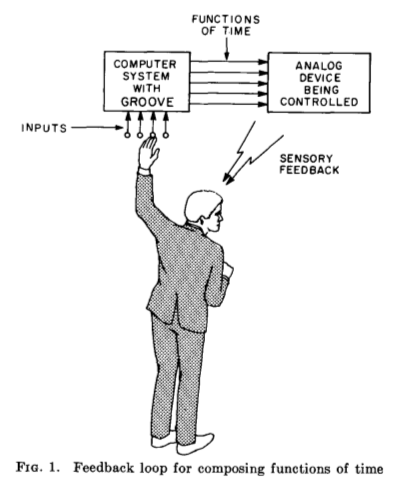
\includegraphics[scale=0.5]{./imagens/GROOVE.png}
\caption{Esquema de concepção do projeto GROOVE descrito no artigo homônimo por Max Mathews \textbf{Fonte}: \cite{mathews_groove_1970}.}
\label{fig:groove_sistema}
\end{center}
\end{figure} 

O terceiro conceito observa a existência de uma relação entre um humano e uma máquina. Mathews descreve-o como uma \emph{engenharia humana}. Esta engenharia consistiu na observação de um tempo diferencial entre o que o(a) musicista cria e o que edita:

\begin{citacao} 
O conceito final é mais nebuloso. Desde que o GROOVE é um sistema homem-máquina, a engenharia humana do sistema foi a mais importante. Por exemplo, nós descobrimos que o controle do programa de tempo necessita ser bastante diferente para a composição do que para a edição, e o programa foi modificado de acordo. (\ldots) O intérprete de computador não deve tentar definir todo o som em tempo real. Ao invés, o computador deve ter uma partitura e o intérprete deve influenciar a forma como a partitura é tocada. Seus modos de influência podem ser mais variados do que aqueles que um regente convencional, que pode principalmente controloar o tempo, intensidade, e estilo.\cite[p.~715-716]{mathews_groove_1970}
\footnote{Tradução nossa de \emph{The final concept is more nebulous. Since GROOVE is a man-computer system, the human engeneering of the system is most important. For example, we discovered that the control of the program time needs to be quite different for composing than for editing, and the program was modiffied accordingly. (\ldots) The computer performer should not attempt to define the entire sound in real-time. Instead, the computer should have a score and the performer should influence the way in which the score is played. His modes of influence can be much more varied than that a conventional conductor who primarily controls tempo, loudness, and style.}.}
\end{citacao}

Como exemplo , selecionamos uma descrição da compositora Laurie \citeonline{spiegel_expanding_1975} (ver \autoref{fig:groove}) para sumarizar as características do GROOVE, durante a produção de \emph{The Expanding Universe} \footnote{Disponível em \url{https://www.youtube.com/watch?v=dYUZmsfm4Ww}.}, entre as salas 2D-506 da Bell Labs (contendo o computador DDP-224) e a sala analógica 2D-562 (laboratório de Mathews). A ``performance'' da obra era realizada, com a programação de funções temporais e a manipulação de parâmetros dessas funções através de dispositivos físicos:

\begin{citacao}
Todas as músicas no GROOVE eram representadas na memória digital como funções abstratas do tempo, séries paralelas de dois pontos, cada ponto sendo um instante no tempo e um valor instantâneo. A taxa de amostragem para essas funções, usada principalmente como controle de voltagem, era cronometrada por um grande e antiquado oscilador analógico que era normalmente fixado em 100 Hertz, cada ciclo do oscilador pulsando à frente do código, o computador lia, em cada uma das funções, naquele ponto do tempo, todos dispositivos de entrada e executava todas amostras. (\ldots) Tínhamos uma pequena caixa com 4 potenciômetros e quatro chaves (alternadores fixados onde você os colocava) e dois botões de disparo.\footnote{Tradução de \emph{All music in GROOVE was represented in digital memory as abstract functions of time, parallel series of point pairs, each point being an instant in time and an instantaneous value. The sampling rate for these functions, which would be used mostly as control voltages, was clocked by a big old-fashioned analog oscillator that was usually set to 100 Hertz, each cycle of the oscillator pulsing one run through the code, the computer reading all of the real time input devices and playing of all of the samples at that time point in each of the time functions. (\ldots)  We had a small box with 4 knobs, 4 set switches (toggles that stay where you put them) and 2 momentary-contact push buttons on it.}}
\end{citacao}

\begin{figure}[!h]
  \begin{center}
  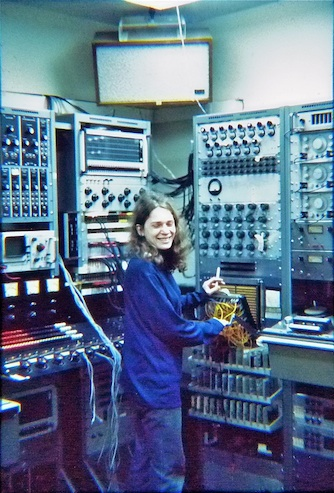
\includegraphics[scale=0.5]{./imagens/spiegel.jpg}
  \caption{\small Laurie Spiegel configurando a saída analógica do GROOVE, durante a produção de \emph{The Expanding Universe}. \textbf{Fonte}: \cite{spiegel_expanding_1975}.}
  \label{fig:groove}
  \end{center}
\end{figure}

Embora não declare ser uma peça minimalista, a descrição de \emph{The Expanding Universe} considera, de maneira asséptica, os fenômenos psicoacústicos como elementos composicionais. Por exemplo, a utilização da continuidade progressiva de sons (ou \emph{drones} transitórios) como elemento criativo permite, segundo a compositora, à sensibilização do ouvido, o que não seria possível na música minimalista instrumental:

\begin{citacao}
 A violência da perturbação sonora, disjunção, descontinuidade e mudanças súbitas desanitizam o ouvinte e nos afastam, de forma que não estamos mais abertos aos sons mais sutis. Mas com continuidade e gentileza, o ouvido se torna re-sensibilizado para mais e mais fenômenos auditoriais sutis dentro do som que estamos imersos. Em vez de sermos arrastados, como nas cascatas de muitas notas executadas em blocos de tempo que mudam repentinamente, tal como tantas vezes consite a música "minimalista", abrimos nossos ouvidos mais e mais para os mais fenômenos que nos envolvem. Isto também não é música ambiente, um termo que veio a ser usado alguns anos depois. Esta é música para atenção concentrada, uma experiência musical do através, pensando que, lógico, existe também um pano de fundo. \footnote{Tradução de\emph{The violence of sonic disruption, disjunction, discontinuity and sudden change desensitizes the listener and pushes us away so we are no longer open to the subtlest sounds. But with continuity and gentleness, the ear becomes increasingly re-sensitized to more and more subtle auditory phenomena within the sound that immerses us. Instead of being swept along, as with cascades of many running notes in suddenly-changing blocks of time, such as “minimalist” music so often consists of, we open up our ears more and more to the more minute phenomena that envelope us. This is also not “ambient music”, a term that came into use some years later. This is music for concentrated attention, a through-composed musical experience, though of course it also can be background.}}
\end{citacao}

Nesta citação podemos sumarizar um conceito para o \emph{live coding}: processo. Porém, o significado de processo pode ser desenvolvido infinitamente. Isso não será realizado. O significado de processo para Spiegel é diverso daquele considerado no \emph{live coding}, e uma digressão desta pode afastar demais o foco do trabalho principal. Para compreender o significado de processo no \emph{live coding}, será necessário continuar.

\subsection{Pietro Grossi}\label{sec:grossi}

Embora pouco conhecido no contexto geral da música européia, o compositor Pietro Grossi foi  um dos pioneiros da \emph{Computer Music} Italiana. O pensamento musical que rege seus programas de computador sacrifica questões timbrísticas para concentrar na performance. O primeiro \emph{software} desenvolvido foi o DCMP (\emph{Digital Computer Music Program}) e, segundo \cite{mori_pietro_2015}, ao usar este programa,

\begin{citacao}
(\ldots) o intéprete era capaz de produzir e reproduzir música em tempo real, digitando alguns comandos específicos e os parâmetros composicionais desejados. O som resultante vinha imediatamente depois da operação de decisão, sem qualquer atraso causado por cálculos. Haviam muitas escolhas de reprodução no programa: era possível salvar na memória do computador peças de músicas pré-existentes, para elaborar qualquermaterial sonoro no disco rígido, para administrar arquivos musicais e iniciar um processo de composição automático, baseado em algoritmos que trabalham com procedimentos ``pseudo-casuais''. Exsitia também uma abundância de escolhas para mudanças na estrutura da peça. Um dos mais importantes aspectos do trabalho de Grossi foi que todas intervenções eram instantâneas: o operado não tinha que esperar pelo computador terminar todas operações requisitadas, e depois ouvir os resultados. Cálculos de dados e reprodução sonoras eram simultâneos. Esta simultaneidade não era comum no campo da \emph{Computer Music} daquele tempo, e Grossi deliberadamente escolheu trabalhar desta forma, perdendo muito no lado da qualidade sonora. Seu desejo era poder escutar os sons resultantes imediatamente. \cite[p.~126]{mori_pietro_2015} \footnote{Tradução nossa de \emph{(\ldots) the performer was able to produce and reproduce music in real time by typing some specific commands and the desired composition's parameters. The sound result came out immediately after the operator's decision, without any delay caused by calculations. There were many reproduction choices inscribed in this software: it was possible to save on the computer memory pieces of pre-existing music, to elaborate any sound material in the hard disk, to manage the music archive and to start an automated music composition process based on algorithms that worked with “pseudo-casual” procedures. There were also plenty of choices for piece structure modifications. One of the most important aspects of Grossi’s work was that all the interventions were instantaneous: the operator had not to wait for the computer to finish all the requested operations and then hear the results. Data calculation and sound reproduction were simultaneous. This simultaneity was not common in the computer music field of that time and Grossi deliberately chose to work in this way, losing much on the sound quality’s side. His will was to listen to the sound result immediately.}}
\end{citacao}

Esta abordagem parte de uma abordagem ``preguiçosa'' (\emph{lazy}). Grossi dizia sobre si mesmo, como ``uma pessoa que está consciente de que o seu tempo é limitado e não quer perder tempo em fazer coisas inúteis ou na espera de alguma coisa quando não é necessário.''\footnote{Tradução nossa de \emph{a person who is aware that his or her time is limited and do not want to waste time in doing useless things or in waiting for something when it is not necessary.}}. Neste sentido, defendia que o desenvolvimento de novos timbres deveria esperar por melhores implementações de \emph{hardware}.

O sacrifício do timbre reflete a utilização o computador como uma paródia do piano, ou até mesmo de um violino. Grava em 1967 ``Mixed Paganini''\footnote{Disponível em \url{https://www.youtube.com/watch?v=ZQSP_wF7wSY}.}, uma execução ultra-virtuosística dos \emph{Capricci op.1} de Niccolò Paganini; foi executada no computador Olivetti GE-115 \citeonline[p.~126]{mori_pietro_2015}.

Sumarizamos o seguinte conceito: \emph{reflexividade}, ou a \traducao{habilidade de um de um programa manipular como dados algo que representa o estado do programa durante sua própria execução, o mecanismo para codificação de estados de execução é chamado \emph{reificação}.\cite[p.~1]{malefant_reflection_1996}}{the ability of a program to manipulate as data something representing the state of the program during its own execution, the mechanism for encoding execution states as data being called reification.}

\subsubsection{Just In Time (JIT)}\label{sec:jit}

A reflexividade é uma característica de diversos ambientes de \emph{live coding}. O \emph{SuperCollider} foi o primeiro dos ambientes de programação musical a implementar esta caracterísitca, a partir da tecnologia \emph{Just In Time Compilation} (Compilação JIT)

Segundo \citeonline{aycock_brief_2003}, o primeiros programas JIT foram Genesis (com base no LISP, 1960), LC$^2$ (\emph{Language for Conversational Computing}, 1968) e APL (1970). Este último tinha duas novidades técnicas, a partir dos termos \emph{drag-along} e \emph{beating}; estes são hoje chamados de \emph{lazy evaluation} (avaliação preguiçosa). 

Atualmente, esta técnica têm sido largamente implementada para navegadores de internet \cite{roberts_web_2013}. Programas como Gibber\footnote{Disponível em \url{http://gibber.mat.ucsb.edu/}.} \cite{roberts_gibber:_2012} e \emph{wavepot}\footnote{Disponível em \url{https://www.wavepot.com}.} são exemplares; permitem a agregação do conceito de \emph{reflexividade} ao conceito \emph{redes}, que será apresentado na próxima seção.

%Durante a pesquisa, desenvolvemos em parceria com o pesquisador Flávio Schiavonni um ambiente JIT para síntese sonora, inspirado no GROOVE.


\subsection{Baía de São Franscisco}\label{sec:baiasaofranscisco}

\traduzcitacao{Com o florescimento da indústria de computadores pessoais na Baía de São Franscisco, o acesso às novas tecnologias e pessoas que desenvolveram elas era talvez o melhor no mundo. Mas se para todos os jovens com fortunas como panos para suas mentes (e seus futuros) que perseguiam um excitamento aditivo na construção de máquinas eletrônicas, também existiam políticos utópicos que sonhavam com uma nova sociedade construída no livre e aberto acesso à informação, e na abrangente tecnologia baseada em sistemas inteligentes. Esta também é a cultura que deu ao mundo a música ``New Age'', uma versão aguada e comercializada das músicas com base em modos e drones que Terry Riley, Pauline Oliveros, e LaMonte Young inventaram durante os anos cinquenta e sessenta. Mas a música da Costa Oeste também incluía livre-restrição, barulho, e improvisações com bordas que sobraram das revoluções contra-culturais dos anos 60}{With the flowering personal computer industry in the Bay Area, access to the new digital technologies and to the people who developed them was perhaps the best in the world. But for all the young men with fortunes in the back of their minds (and in their futures) who pursued the addictive excitement of building electronic machines, there were also the political utopians whose dream was of a new society built on the free and open access to information, and on a comprehensively designed technology based on embedded intelligence. This was also the culture that gave the world "New Age" music, a watered-down and commercialized version of the musics based on modes and drones that Terry Riley, Pauline Oliveros, and LaMonte Young invented here during the late fifties and early sixties. But West Coast music-making also included a free-wheeling, noisy, improvisational edge left over from the counter-cultural revolutions of the sixties.}{online}{brown_indigenous_2013}

Na segunda metade da década de setenta, Jim Horton começou a adquirir micro-controladores KIM-1\footnote{Disponível em \url{http://www.6502.org/trainers/buildkim/kim.htm}.}. Segundo \citeauthoronline{brown_indigenous_2013}, não demorou para que outros interessados comprassem. Discussões informais posteriores, que incluiam, além de Horton, David (Behrman), John Bischoff, Tim Perkis, Rich Gold, Cathy Morton, Paul Robinson, e Paul Kalbach, sugeria a formação de uma ``orquestra de silício'' (\emph{silicon orchestra}).

Ademais, em 1977, Horton colaborou com duas peças que interligavam estes microcontroladores. A primeira era construída sobre algoritmos inspirados nas teorias matemáticas de Leonard Euler (séc. XVIII). A segunda peça também explorava a comunicação entre os microcontroladores, de forma que \traducao{notas ocasionais da minha (Bischof) máquina faziam a máquina de Jim transpor atividades melódicas de acordo com minha nota base\cite[online]{brown_indigenous_2013}}{the occasional tones of my machine caused Jim’s machine to transpose its melodic activity according to my "key" note. }.

Em 1978, Bischof, Behrman, Gold e Horton gravaram um \emph{Extended Play} (EP)\footnote{Gravação muito longa para um \emph{demo} e insuficiente para um disco, de vinil na época.} a partir de uma performance em 26 de Novembro de 1978, lançado pela pela Lovely Music (NY) em 1980 como \emph{The Hub: Computer Network Music}. Durante este tempo, foi formado o grupo \emph{``The League of Automatic Music Composers''}, que além de  Bischof, Perkis, Brown, contava com Scot Gresham-Lancaster, Mark Trayle e Phil Stone. Aquele era um momento onde os \emph{happenings} já eram manifestações artísticas consolidadas. Não demorou muito para que o público participasse da atividade:

\begin{citacao}
Na primavera de 1979, montamos uma série quinzenal regular de apresentações informais sob os auspícios da \emph{Bay Center for the Performing Arts}. Todos outros domingos à tarde passávamos algumas horas configurando nossa rede de KIMs na sala \emph{Finnish Hall}, na Berkeley, e deixávamos a rede tocando, com retoques aqui e ali, por uma ou duas horas. Os membros da audiência poderiam ir e vir como quisessem, fazer perguntas, ou simplesmente sentar e ouvir. Este foi um evento comunitário de tipos como outros compositores aparecendo, tocando ou compartilhando circuitos eletrônicos que tinham projetado e construído. Um interesse na construção de instrumentos eletrônicos de todos os tipos parecia estar "no ar". Os eventos da sala \emph{Finn Hall} foram feitos para uma cena com paisagens sonoras geradas por computador misturado com os sons de grupos de dança folclórica ensaiando no andar de cima e as reuniões ocasionais do Partido Comunista na sala de trás do edifício velho venerável. A série durou cerca de 5 meses que eu me lembre.\cite[online]{brown_indigenous_2013}\footnote{Tradução nossa de: \emph{In the spring of 1979, we set up a regular biweekly series of informal presentations under the auspices of the East Bay Center for the Performing Arts. Every other Sunday afternoon we spent a few hours setting up our network of KIMs at the Finnish Hall in Berkeley and let the network play, with tinkering here and there, for an hour or two. Audience members could come and go as they wished, ask questions, or just sit and listen. This was a community event of sorts as other composers would show up and play or share electronic circuits they had designed and built. An interest in electronic instrument building of all kinds seemed to be "in the air." The Finn Hall events made for quite a scene as computer-generated sonic landscapes mixed with the sounds of folk dancing troupes rehearsing upstairs and the occasional Communist Party meeting in the back room of the venerable old building. The series lasted about 5 months as I remember.}}
\end{citacao}

Nesta seção sumarizamos os conceito \emph{rede de composições}. Este conceito pode ser melhor compreendido através de uma descrição do processo criativo da banda:

\traduzcitacao{Os membros da liga geralmente adaptavam composições solo para usar dentro da banda. Estes solos eram desenvolvidos independentemente por cada compositor, e eram tipicamente baseados em esquemas de algoritmos de um tipo ou outro. Existiam características de improvisação diferentes para muitas delas, como bem as músicas eram diferentes em detalhes. Teorias matemáticas sistemas de afinação experimentais, algoritmos de inteligência artificial, projetos de instrumentos de improvisação, e performance interativa eram algumas das áreas exploradas nestes trabalhos (\ldots) Os solos tocavam simultaneamente no cenário de grupo, se tornando ``sub''-composições que interagem, cada uma enviando e recebendo dados pertinentes para o funcionamento musical}
{League members generally adapted solo compositions for use within the band. These solos were developed independently by each composer and were typically based on algorithmic schemes of one kind or another. There was a distinctly improvisational character to many of these as the music was always different in its detail. Mathematical theories of melody, experimental tuning systems, artificial intelligence algorithms, improvisational instrument design, and interactive performance were a few of the areas explored in these solo works. (\ldots) The solos, played simultaneously in the group setting, became interacting "sub"-compositions, each sending and receiving data pertinent to its musical functioning.}
{online}
{brown_indigenous_2013}


\subsection{Ron Kuivila}

Segundo \citeonline{mclean_patterns_2009}, Ron Kuivila realiza a primeiras performance de \emph{live coding} em 1985 com a performance \emph{Water Surfaces} na STEIM\footnote{\emph{STudio for Electro-Instrumental Music}, disponível em \url{http://steim.org/about/}.}, em Amsterdã \cite{blackwell_programming_2005}. 

O disco ``\emph{TOPLAP001 - A prehistory of live coding}'' traz uma reconstrução da peça realizada em 2007 \footnote{Disponível em \url{http://toplap.org/wiki/TOPLAP_CDs}.}; uma nota sobre a performance descreve o seguinte: \traducao{Esta obra usou programação FORTH ao vivo; Curtis Roads testemunhou e relatou a performance de Ron Kuivila feita na STEIM em Amsterdã, em 1985; a performance original termina com a quebra do sistema.}{This work used live FORTH programming; Curtis Roads witnessed and reported a performance by Ron Kuivila at STEIM in 1985; the original performance apparently closed with a system crash\ldots}\footnote{FORTH é uma linguagem de programação elaborada por Charles Moore (1938-). Entre seus paradigmas de programação, utiliza da \emph{reflexividade}.}. 

Ge \citeonline{wang_historical_2005}, em uma comunicação pessoal com Curtis Roads, cita a seguinte declaração: \traducao{Eu vi o \emph{software} FORTH de Ron Kuivila quebrar e queimar no palco em Amsterdã em 1985, mas antes disso, não fez uma música muito interessante. A performance consistiu de digitação}{I saw Ron Kuivila's Forth software crash and burn onstage in Amsterdam in 1985, but not before making some quite interesting music. The performance consisted of typing.}

Nenhuma fonte sonora foi encontrada disponível online. Porém este conceito é revisitado por Magno Caliman em \emph{scriptBashing} (2015): a recodificação de um programa escrito em linguagem C cria centenas (na ordem de 800) processos paralelos só no plano visual. Outros processos, com a criação de sintetizadores no SuperCollider, embora parcialmente visíveis, são adicionados na pilha de memória. A performance acaba com um silêncio decorrente da saturação da memória RAM.


\subsection{Live Algorithm Programming and Temporary Organization for its Promotion}\label{sec:laptoptoplap}

Este acrônimo deriva  do manifesto ``\emph{Live Algorithm Programming and Temporary Organization for its Promotion}'', LAPTOP, \cite{ward_live_2004,blackwell_programming_2005}.

No \emph{Wiki} do site oficial\footnote{Disponível em \url{http://toplap.org/wiki/Main_Page}.}, a cada visita, a ordem das letras são permutadas, criando diferentes significados. Por exemplo, \emph{Transdimensional Organisation for the Pragmatics of Live Algorithm Programming}, \emph{Terrestrial Organisation for the Proliferation of Live Artistic Programming}, \emph{Temporal Organisation for the Proliferation of Live AudioVisual Programming} e outros. 

Este comportamento, de permutar ordem das letras, de algum título, ou até mesmo do próprio nome para gerar pseudônimos, já era praticada por Click Nilson (Nick Collins), que define bem o \emph{live coding}: \traducao{Live coding celebra a efemeralidade de sua própria definição}{Live coding celebrates the ephemerality of definition itself. Disponível em \url{http://lurk.org/groups/livecode/messages/topic/ofAxZpxsKFpDRLnoA48Bh}.}

Este manifesto expõe os ambientes de performance, bem como alguns ritos técnicos do improvisador. Espaços de Música Eletrônica de Pista se misturam com a Música algorítmica e a Música de processos:

\begin{citacao}
O \emph{Livecoding} permite a exploração de espaços algorítmicos abstratos como uma improvisação intelectual. Como uma atividade intelectual, pode ser colaborativa. Codificação e teorização podem ser atos sociais. Se existe um público, revelar, provocar e desafiar eles com uma matemática complexa se faz com a esperança de que sigam, ou até mesmo participem da expedição. Estas questões são, de certa forma, independentes do computador, quando a valorização e exploração de algoritmo é que importa. Outro experimento mental pode ser encarado com um DJ ao vivo codificando e escrevendo uma lista de instruções para o seu \emph{set} (realizada com o iTunes, mas aparelhos reais funcionam igualmente bem). Eles passam ao HDJ $[$ \emph{Headphone Disk Jockey} $]$ de acordo com este conjunto de instruções, mas no meio do caminho modificam a lista. A lista está em um retroprojetor para que o público possa acompanhar a tomada de decisão e tentar obter um melhor acesso ao processo de pensamento do compositor. \cite[p.~245]{ward_live_2004} \footnote{Tradução nossa de: \emph{Live coding allows the exploration of abstract algorithm spaces as an intellectual improvisation. As an intellectual activity it may be collaborative. Coding and theorising may be a social act. If there is an audience, revealing, provoking and challenging them with the bare bone mathematics can hopefully make them follow along or even take part in the expedition. These issues are in some ways independent of the computer, when it is the appreciation and exploration of algorithm that matters.   Another thought experiment can be envisaged in which a live coding DJ writes down an instruction list for their set (performed with iTunes, but real decks would do equally well). They proceed to HDJ according to this instruction set, but halfway through they modify the list. The list is on an overhead projector so the audience can follow the decision making and try to get better access to the composer’s thought process.}}
\end{citacao}

O trecho acima fornece informações a respeito do espaços conceitual do \emph{algorave}, ou das pŕaticas de \emph{Disk Jockey} com a utilização da a atividade de programação em linguagem de computador. Adiante podemos ver outros dois conceitos aglutinados: Música de Processos, ou Música de algoritmos simples, e Música Generativa \footnote{Para mais informações, ver \citeonline{reich_music_1968} e \citeonline[p.~128]{mailman_agency_2013}. Sobre Música generativa, \citeonline{eno_generative_1996} }:

\begin{citacao}
Contudo, alguns músicos exploram suas idéias como processos de \emph{software}, muitas vezes ao ponto que o \emph{software} se torna a essência da música. Neste ponto, os músicos podem ser pensados como programadores explorando seu código manifestado como som. Isso não reduz seu papel principal como um músico, mas complementa, com a perspectiva única na composição de sua música. \textbf{Termos como ``música generativa'' e ``música de processos'' tem sido inventados e apropriados para descrever esta nova perspectiva de composição}. Muita coisa é feita das supostas propriedades da chamada ``música generativa'' que separa o compositor do resultado do seu trabalho. Brian Eno compara o fazer da música generativa com o semear de sementes que são deixadas para crescer, e sugere abrir mão do controle dos nossos processos, deixando eles ``brincarem ao vento''. \footnote{\opcit[p.~245-246]{ward_live_2004}. Tradução nossa de \emph{Indeed, some musicians explore their ideas as software processes, often to the point that a software becomes the essence of the music. At this point, the musicians may also be thought of as programmers exploring their code manifested as sound. This does not reduce their primary role as a musician, but complements it, with unique perspective on the composition of their music. Terms such as “generative music” and “processor music” have been invented and appropriated to describe this new perspective on composition. Much is made of the alleged properties of so called “generative music” that separate the composer from the resulting work. Brian Eno likens making generative music to sowing seeds that are left to grow, and suggests we give up control to our processes, leaving them to “play in the wind”.}}
\end{citacao}

\subsubsection{\emph{Algoraves}}\label{sec:algorave}

Algorave é  um tipo de música eletronica de pista, que se utiliza de algoritmos, processos, e teorias generativas; seus processos criativos replicam alguns regimes de escuta, tais como \emph{dance}, \emph{drum'n'bass}, \emph{cyberpunk}. No entanto, \emph{algorave} é um termo anterior ao advento do \emph{live coding}: 

\begin{citacao}
\emph{Algorave} não é sustentado exclusivamente por \emph{live coders}, mas estes têm mantido uma forte presença em todos os eventos até agora. É assim talvez, porque a tradição do \emph{live coding} de projetar telas motiva todo o esforço; onde algoritmos não estão visíveis por períodos de tempo durante uma algorave, se corre o risco das coisas parecerem muito como um evento de música eletrônica padrão. \cite[p.~356]{collins_algorave:_2014} \footnote{Tradução nossa de \emph{Algorave is not exclusively a preserve of live coders, but they have maintained a strong presence at every event thus far. This is perhaps because the live coding tradition of projecting screens help motivates the whole endeavour; where algorithms are not made visible for periods during an algorave, we run the risk of things feeling much like a standard electronic music event.}}
\end{citacao}


\citeonline{collins_algorave:_2014} apresentam dados a respeito da história da \emph{algorave}, de 1992 a 2004. Em 1992, Charles Ames disponibiliza o \emph{Cybernetic Composer}, \traducao{um \emph{software} com um sistema baseado em Inteligência Artificial que compõe música em uma variedade de estilos populares.}{an AI based software system that composes music in a variety of popular styles.}\footnote{Disponível em \url{http://www.kurzweilai.net/charles-ames}}. Em 1994, o duo \emph{Koan}, formado pelos DJs Daniel Roeth e William Grey, realizam adaptações para entretenimento com base no \emph{ambient music} de Brian \citeonline{eno_music_1978}. \emph{Aphex Twin} (Richard David James) reinvindica em 1997 o termo \emph{live club algorithm}. Em 1999, o protocolo para edição audiovisual ao vivo \emph{bbcut} \cite{collins_bbcut_2003} é incluído nos \emph{opcodes} do \emph{CSound}\footnote{Disponível em \url{https://csound.github.io/}.}, e do \emph{Supercollider}. Em 2000 o \emph{Slub}, realizam performances, autodenominadas \emph{generative techno}, com abordagem \emph{gabba}. Em 2001 é identificado a utilização de redes neurais para composição de padrões semelhantes ao \emph{drum'n'bass}. Em 2004 é fundado o TOPLAP, organização internacional  de \emph{live coding}, em uma casa noturna de Hamburgo. \footnote{\loccit{collins_algorave:_2014}.}

De maneira sumarizada, escolhemos os conceitos: \emph{música de processos, música generativa, Inteligência Artifical, e música de pista} como conceitos relacionados ao manifesto ``\emph{Live Algorithm Programming and Temporary Organization for its Promotion}''.

\subsection{\emph{Show us your screens}}\label{sec:showusyourscreens}

Além das performances inaugurais nos festivais Europeus, e do manifesto ``Live Algorithm Programming and Temporary Organization for its Promotion'', ``\emph{Show Us Your Screens}''  \cite[p.~22; online]{griffiths_fluxus:_2008,mccallum_show_2011}, contêm as regras heurísticas do \emph{live coding}:

\begin{citacao}
Exigimos:

• Acesso à mente do intérprete, para todo o instrumento humano.

• Obscurantismo é perigoso. Mostre-nos suas telas.

• Programas são instrumentos que podem modificar eles mesmos.

• O programa será transcendido - Língua Artificial é o caminho.

• O código deve ser visto assim como ouvido, códigos subjacentes visualizados bem como seu resultado visual.

• Codificação ao vivo não é sobre ferramentas. Algoritmos são pensamentos. Motosserras são ferramentas. É por isso que às vezes algoritmos são mais difíceis de perceber do que motosserras.

Reconhecemos contínuos de interação e profundidade, mas preferimos:

• Introspecção dos algoritmos.

• A externalização hábil de algoritmo como exibição expressiva/impressiva de destreza mental.

• Sem \emph{backup} (minidisc, DVD, safety net computer).

Nós reconhecemos que:

• Não é necessário para uma audiência leiga compreender o código para apreciar, tal como não é necessário saber como tocar guitarra para apreciar uma performance de guitarra.

• Codificação ao vivo pode ser acompanhada por uma impressionante exibição de destreza manual e a glorificação da interface de digitação.

• Performance envolve contínuos de interação, cobrindo talvez o âmbito dos controles, no que diz respeito ao parâmetro espaço da obra de arte, ou conteúdo gestual, particularmente direcionado para o detalhe expressivo. Enquanto desvios na tradicional taxa de reflexos táteis da expressividade, na música instrumental, não são aproximadas no código, por que repetir o passado? Sem dúvida, a escrita de código e expressão do pensamento irá desenvolver suas próprias nuances e costumes.
\footnote{Tradução nossa de:\emph{We demand: \begin{inparaenum}[•]
\item Give us access to the performer's mind, to the whole human instrument.
\item Obscurantism is dangerous. Show us your screens.
\item Programs are instruments that can change themselves.
\item The program is to be transcended - Artificial language is the way.
\item Code should be seen as well as heard, underlying algorithms viewed as well as their visual outcome.
\item Live coding is not about tools. Algorithms are thoughts. Chainsaws are tools. That's why algorithms are
sometimes harder to notice than chainsaws.
\end{inparaenum}. We recognise continuums of interaction and profundity, but prefer:  \begin{inparaenum}[•]
\item Insight into algorithms
\item The skillful extemporisation of algorithm as an expressive/impressive display of mental dexterity
\item No backup (minidisc, DVD, safety net computer)
\end{inparaenum}. We acknowledge that: \begin{inparaenum}[•]
\item It is not necessary for a lay audience to understand the code to appreciate it, much as it is not necessary
to know how to play guitar in order to appreciate watching a guitar performance.
\item Live coding may be accompanied by an impressive display of manual dexterity and the glorification of the
typing interface.
\item Performance involves continuums of interaction, covering perhaps the scope of controls with respect to
the parameter space of the artwork, or gestural content, particularly directness of expressive detail. Whilst
the traditional haptic rate timing deviations of expressivity in instrumental music are not approximated in
code, why repeat the past? No doubt the writing of code and expression of thought will develop its own
nuances and customs.
\end{inparaenum}}}
\end{citacao}

``Dar acesso à mente do intérprete'' e ``obscurantismo é perigoso'' descrevem um meio de evitar qualquer código mal intencionado; isto é uma hipótese: \begin{inparaenum}[\itshape i)\upshape]
\item programas de \emph{live coding} geralmente são programas em fase de desenvolvimento;
\item programas em desenvolvimento possuem, inevitavelmente, \emph{bugs}\footnote{Segundo James S. Huggins, historicamente ``O termo \emph{bug} é usado de forma limitada para designar qualquer falha ou problema em conexões ou no trabalho com aparatos elétricos'' Tradução nossa de \emph{The term "bug" is used to a limited extent to designate any fault or trouble in the connections or working of electric apparatus.} (ver \url{http://www.jamesshuggins.com/h/tek1/first_computer_bug.htm}). Nesse sentido, um \emph{bug} em um programa é uma falha de operação, geralmente causada por algum erro de lógica, por parte do programador.}
\item \emph{bugs} podem ser explorados e levar à corrupção do sistema.
\end{inparaenum} Se esta hipótese estiver correta, justificaria a atitude de exposição da \emph{imagem-texto}. No entanto não encontrei algum estudo crítico descrevendo se isso é verdade a partir do ponto de vista do público, isto é, será que o público pode estar realmente interessado na exposição da \emph{imagem-texto}? Será que essa exposição não pode ser perigosa para o processo artístico e para a experiência do público? Embora sejam questões que fogem do escopo do trabalho, são importantes, necessitando verificar algumas performances para averiguar.

``Programas são instrumentos'' e ``O programa será transcendido - Língua Artificial é o caminho'', são frases que fazem menção direta à experiência de usuário (\emph{live coder}), isto é, um sistema que é programável de maneira facilitada. A seguinte hipótese pode ser feita: quanto mais simplificada a linguagem de programação, mais expressão visual ou musical um espetáculo poderá ter (o que pode não ser verdade, e sim que a expressão musical estaria no nível sensível). Por ``Língua Artifical'' entendo que o \emph{live coder} pode criar \emph{mini-linguagens} ou Linguagens de Domínio Específico (DSL)\footnote{Sobre esse tema recomendo o texto ``Minilanguages, finding a notation that sings'' de \citeonline{raymond_minilanguages_2003}: ``Historicamente, linguagens de dominio especifico sao do tipo que sao chamadas de 'pequenas linguagens' ou 'minilinguagens' no mundo do Unix, porque os primeiros exemplos eram pequenos e de pouca complexidade, em relaçao às linguagens de propósito geral (\ldots) Nós manteremos o termo tradicional 'minilinguagem'para engatizar que no decorrer do curso é geralmente utilizado para projetar e mantê-las o menor e simples possível'' \cite[$3^o$ parágrafo]{raymond_minilanguages_2003}. Tradução nossa de \emph{Historically, domain-specific languages of this kind have been called ‘little languages’ or ‘minilanguages’ in the Unix world, because early examples were small and low in complexity relative to general-purpose languages (\ldots) We'll keep the traditional term ‘minilanguage’ to emphasize that the wise course is usually to keep these designs as small and simple as possible.}} que possibilitam criar programas para criar um espetáculo audiovisual ou musical. Segundo \citeonline{collins_algorave:_2014}, tais DSLs estariam no formato de ``mini-linguagens'' bem desenvolvidas para a tarefa específica de codificar música ao vivo, operando técnicas composicionais como a transformação de um padrão musical (como por exemplo, técnicas barrocas como inversão e retrogradação ou técnicas aleatórias, como emabaralhamento de um conjunto de eventos sonoros), facilitando a espontaneidade no processo criativo:

\begin{citacao}
Existe um número crescente de sistemas de \emph{livecoding} com ``mini-linguagens'' amigáveis, que facilitam o \emph{loop} e contruções de camadas centrais típicas para dançar música. \emph{Ixilang} é um exemplo primário, e possui um editor de código estruturado que, enquanto baseado em texto, suporta correspondências visuais. \emph{Tidals} é outro, e, embora com foco na rapidez de utilização ao invés da facilidade de aprendizagem, está começando a ter mais ampla aceitação. Ambos \emph{ixilang} e \emph{Tidal} promovem padrões em termos de funções transformadoras como embaralhamento, inversão e extrapolação de formas diferentes.  \cite[p~.357]{collins_algorave:_2014}\footnote{Tradução nossa de: \emph{There are increasingly user friendly “mini-language” livecoding systems which facilitate loop and layer-centric con-structions typical to dance music. ixilang is a primary example, and features a structured code editor which while text-based, supports visual correspondences. Tidal is another, and although its focus is on speed of use rather than ease of learning, is beginning to see wider take-up. Both ixilang and Tidal promote pattern in terms of transformative functions as scrambling, reversal and extrapolation in different ways}.}
\end{citacao}


``O código deve ser visto assim como ouvido'' entraria em um problema próprio de programas de pesquisa em notação musical, sendo que o processo de correlação entre o que está escrito e o que está sendo ouvido leva um tempo ou pode mesmo nem existir. Mesmo com o convite expressado pelo manifesto ``\emph{Live Algorithm Programming and Temporary Organization for its Promotion}'' no início do capítulo, a questão não está nem no uso do computador nem em alguma abordagem musical, e conforme a performance avança, a imagem-texto vai se tornando tão poluída que poderia causar um desinteresse.

\begin{citacao}
Codificação e teorização podem ser atos sociais. Se existe um público, revelar, provocar e desafiar eles com uma matemática complexa se faz com a esperança de que sigam, ou até mesmo participem da expedição. Estas questões são, de certa forma, independentes do computador, quando a valorização e exploração de algoritmo é que importa.\cite[p.~204]{ward_live_2004}
\end{citacao}

``Algoritmos são pensamentos. Motosserras são ferramentas.'', ``Introspecção dos algoritmos.'' e ``A externalização hábil de algoritmo'' descrevem uma atividade constante de formalizações lógicas, do processo febril de explorar uma complexidade própria do que se criou, de ficar digitando sem parar um teclado de computador. Alguns colegas e amigos não programadores, músicos e não músicos, utilizam a expressão ``gostar de apertar botão'' para se referir à caricatura do programador em um espaço reservado, no qual controla dispositivos diversos.

``Sem \emph{backup}'' indica o comportamento do \emph{live coder} após uma improvisação, que não memoriza em discos rígidos, cd's ou \emph{pendrives} o documento criado (isto é, o código textual, em alguma extensão apropriada para a linguagem utilizada, por exemplo, \emph{.pl}, Perl, \emph{.scheme}, Scheme, \emph{.js}, JavaScript), da mesma forma que um músico de improvisação dificilmente transcreveria o que tocou em uma partitura, no máximo gravando o áudio da performance.

A respeito de ``Não é necessário para uma audiência leiga compreender'' e ``A codificação ao vivo pode ser acompanhada por uma impressionante exibição de destreza'' pode indicar uma proximidade com aquele modelo de prática musical virtuosística (como um espetáculo de habilidades técnicas); mais especificamente, este modelo poderia partir daquilo que  \citeonline{magnusson_herding_2014} chama de ``adoção de um método pré-romântico de compor através da performance em tempo real, onde tudo fica aberto a mudar -- o processo composicional o design do instrumento e a inteligência do sistema tocando a peça.'' \cite[p.~4]{magnusson_herding_2014}\footnote{Tradução nossa de: \emph{live coding adopts a pre-Romantic method of composing through performance in real time, where everything remains open to change -- the compositional process, the instrument design, and the inteligence of the system performing the piece.}}

%\section{Três apropriações ideológicas}\label{sec:algoritmos}

%Não é nossa intenção discutir a Música de Processos, a Música Algorítmica, e a Música Generativa de maneira pormenorizada, mas sim construir o espaço conceitual para esta pesquisa.  O primeiro conhecimento, a Música de Processos, é incluída de maneira indireta. Será discutido na \autoref{sec:alg_simples}. O segundo conhecimento, é incluído de maneira um pouco mais específica, na \autoref{sec:alg_complexo}. A apropriação de uma prática contemporânea, \emph{Disk Jockey} (DJ), será comentado na \autoref{sec:musica_vanguarda_pista}.


%\subsection{Música de Processos}\label{sec:alg_simples}

%Segundo \citeauthoronline{wooler_framework_2005}, a Música de Processos é uma ``Música resultante de um conjunto de processos colocados em movimento pelo compositor, tais como  'In C' de Terry Rilley e 'It's gonna rain' de Steve Reich'' \apud[p.~1]{wooler_framework_2005}{eno_generative_1996}\footnote{Tradução nossa de \emph{Music resulting from processes set in motion by the composer “In C” by Terry Riley and “Its gonna rain” by Steve Reich}}; o que é chamado de ``procedural'' por \citeauthoronline{wooler_framework_2005}, é chamado por Joshua \citeonline{mailman_agency_2013} em seu artigo ``\emph{Agency, Determinism, Focal Time Frames and Processive Minimalist Music}'', música de processos mínimos, ou música minimalista de processos determinísticos. O autor faz menção aqui ao compositor Alvin Lucier (1931-) e sua peça \emph{Crossings} (1984). Segundo o autor,

%\begin{citacao}
%A longa forma de \emph{Crossings} (1984) de Alvin Lucier é especialmente clara; ela surge processivamente, neste caso de um glissando de som senoidal puro que lentamente (mais de 16 minutos) ascende de infra-sons para a ultra-sons. Um processo discreto combina com este glissando, criando uma série de processos contínuos de curto alcance. Uma orquestra dividida alterna no jogo de alturas consecutivas, em uma escala cromática ascendente ascendente que interage com o glissando. Um grupo inicia e sustenta um intervalo acima daquela do glissando de tal modo que a uma dissonância mútua cria batimentos; conforme o glissando aumenta, a velocidade do batimento diminui; quando se alcança um uníssono com os instrumentos, os batimentos momentaneamente cessam; como o glissando ascende acima da nota dos instrumentos, batimentos gradualmente aceleram. Eventualmente, o outro conjunto entra e sustenta um intervalo de um semitom acima, começando esse processo de curto alcance novamente.\cite[p.~128]{mailman_agency_2013}\footnote{Tradução nossa de \emph{The long-range form of Alvin Lucier’s Crossings (1984) is especially clear; it arises processively, in this case from a glissando of a pure sine tone that slowly (over sixteen minutes) ascends from infrasonic to ultrasonic. A discrete process combines with this glissando, creating a series of short-range continuous processes. A divided orchestra alternates in playing the consecutive pitches of a rising chromatic scale that interacts with the glissando. One ensemble initiates and sustains a pitch just higher than that of the glissando such that their mutual dissonance creates beats; as the glissando rises, the speed of the beats slows; when it reaches a unison with the instruments, the beats momentarily cease; as the glissando ascends above the pitch of the instruments, the beats gradually accelerate. Eventually, the other ensemble enters and sustains a pitch a semitone higher, starting this short-range process again.}}
%\end{citacao}

%Essa descrição é um breve comentário da peça, mas descreve um simples processo de ação musical, bem como relata de forma clara os resultados sonoros. É possível presumir que existe, na execução de \emph{Crossings}, um simples algoritmo que permeia toda a peça: uma alternância de um ritmo lento de dois grupos instrumentais defasados temporalmente em relação ao som emitido pelo alto-falante\footnote{Esse tipo de algoritmo pode ser facilmente implementado em uma linguagem de programação musical, como o SuperCollider (ver \autoref{crossings}).}.

%Uma vez que na MP também é possível notar a influência de um algoritmo, é necessário evitar confusão com o uso original da MP, tal qual em compositores como Reich, Lucier e Riley; já o seu uso apropriado é realizado por Adrian Ward, Julian Rohruber, Frederick Olofsson, Alex McLean, Dave Griffiths, Nick Collins e Amy Alexander. Sugiro portanto comparar o fragmento do manifesto citado na página 53 com um fragmento do manifesto \emph{Music as a Gradual Process} do compositor Steve \citeonline{reich_music_1968}: 

%\begin{citacao}
%O que é distintivo sobre processos musicais é que eles determinam todos detalhes de nota-a-nota (som-a-som) e toda a forma simultaneamente (pense em um \emph{Round} ou um \emph{Canon}). \textbf{Eu estou interessado em processos perceptivos. Eu quero ser capaz de ouvir o processo acontecendo através da música que soa.} Para facilitar a descrição detalhada de um processo musical, a escuta  deve acontecer muito gradualmente. \cite[p.~1]{reich_music_1968}.\footnote{Tradução nossa de: \emph{The distinctive thing about musical processes is that they determine all the note-to-note (sound-to-sound) details and the over all form simultaneously. (Think of a round or infinite canon.) I am interested in perceptible processes. I want to be able to hear the  process happening throughout the sounding music. To facilitate closely detailed listening a musical process should happen extremely gradually. }}
%\end{citacao}

%Quanto ao manifesto de Adrian Ward, Julian Rohruber, Frederick Olofsson, Alex McLean, Dave Griffiths, Nick Collins e Amy Alexande, tenho uma primeira impressão que essa transformação gradual do som não está presente da mesma forma que em Reich, Lucier ou Rilley; vejo que o uso a reminiscência do termo ``processo'' a partir de ``procedural'' e ``processador'' se dá mais pela atividade de reprogramação em uma CGS ou CGC, mais especificamente, para fins de entretenimento. Aqui o \emph{processo} é formalizado como algoritmo, colocado na situação de constante modificação.

%Já no manifesto de Reich o som não é programado, mas se prevê um comportamento musical em constante modificação a partir de uma ação mínima sobre aquilo que produz o som. Um exemplo interessante é seu \emph{Pendulum Music} (1968), onde deixa oscilar microfones posicionados acima de alto-falantes, com os cabos presos no teto; através de um único tipo de ação, restrita apenas pelas distâncias tomadas por intérpretes antes de colocar os microfones em movimento e pela comprimento do cabo preso ao teto\footnote{Seria possível incluir aqui também a resistência do ar ao movimento do objeto.}, ocorrerá um \emph{processo físico} (desaceleração das oscilações que influenciam quando o microfone passará pelo alto-falante) que desencadeará um \emph{processo perceptivo} (escuta de diferentes momentos de quando estes microfones passam pelo alto-falante até um momento estacionário). 

%Tal técnica faz uso deliberado de um fenômeno conhecido como microfonia, um \emph{processo recursivo} onde os sons projetados pelo alto-falante são retro-alimentaados pelo microfone. A retroalimentação já era usada por Pauline \citeonline{oliveros_tape_1969}, como por exemplo em \emph{Beaultifoul Soup} (1967), peça para fita de dois canais, elaborada através de um circuito em retroalimentação (a compositora indica uma atividade musical econômica que ao longo do tempo causa "interessantes mudanças timbrísticas em sons sustentados" \footnote{\cfcite[p.~43]{oliveros_tape_1969} Tradução nossa de: \emph{interesting timbre changes on sustained sounds}}). Uma proposta posterior também foi realizada por Alvin Lucier (1931-) em \emph{I'm sitting in a room} (1969) quando retroalimenta seu próprio discurso em uma sala, incrementando sinais ao gravador, criando um \emph{drone}, ou um som de duração indefinida\footnote{É interessante comentar, nesse contexto, o uso deliberado de \emph{drones} no \emph{livecoding} através de uma apropriação da \emph{Drone Music}.}. Esta técnica de retroalimentação também pode ser utilizada no \emph{live coding}, por exemplo, no SuperCollider (ver \autoref{apendice_delays}).

%\subsection{Música Generativa}\label{sec:alg_complexo}

%Brian Eno foi mencionado por \citeonline{ward_live_2004}, embora a inclusão pareça ser polisêmica. Chamamos  mesmo em um fragmento de texto de \citeonline{eno_music_1978}:

%\begin{citacao}
%O conceito de música projetada especificamente como pano-de-fundo ambiental foi um pioneirismo da indústria Muzak nos anos cinquenta, e tem sido conhecido genericamente como Muzak. As conotações que este termo carrega são particularmente associadas com um tipo de material que as indústria Muzak produz - melodias familiares arranjadas e orquestradas de maneira leve e derivativa. Compreensivelmente, isso leva ouvintes atentos (e compositores) a dispensar inteiramente o conceito de música ambiental como digna de atenção (\ldots) Se as empresas existentes de música enlatada se baseiam em regularizar ambientes cobrindo as idiossincrasias acústicas e atmosféricas, a Música AMbiental intenciona em melhorá-las. \textbf{Se o pano-de-fundo convencional é produzido removendo todo o sentido de dúvida e incerteza (e portanto o interesse genuíno) da música, a Música Ambiental retém essas qualidades} \cite[online]{eno_music_1978}\footnote{\emph{The concept of music designed specifically as a background feature in the environment was pioneered by Muzak Inc. in the fifties, and has since come to be known generically by the term Muzak. The connotations that this term carries are those particularly associated with the kind of material that Muzak Inc. produces - familiar tunes arranged and orchestrated in a lightweight and derivative manner. Understandably, this has led most discerning listeners (and most composers) to dismiss entirely the concept of environmental music as an idea worthy of attention.(\ldots)Whereas the extant canned music companies proceed from the basis of regularizing environments by blanketing their acoustic and atmospheric idiosyncracies, Ambient Music is intended to enhance these. Whereas conventional background music is produced by stripping away all sense of doubt and uncertainty (and thus all genuine interest) from the music, Ambient Music retains these qualities.} Grifo nosso.}
%\end{citacao} 

%É interessante que neste contexto podemos fazer referência à \emph{Discreet Music} (1975) e \emph{Ambient 1: Music for Airports} (1978); tais peças fazem uso deliberado de laços de fitas que criam sistemas de atrasos (\emph{delays}). Se tais procedimento criativos não eram novos na época \footnote{Nesse sentido indicamos as peças de Steve Reich e Alvin Lucier e Pauline Oliveros já citadas.}; geralmente essas abordagens podem criar \emph{drones} que ficam variando em seu espectro.

%Um exemplo interessante de \emph{live coding} com \emph{drones}, que utiliza pequenos impulsos sonoros no SuperCollider (ver \autoref{sc_drone}). Aqui o processo de escuta é contínuo, semelhante à práticas da música eletroacústica,onde algoritmos são pré-concebidos e modificados durante a performance.  Cole Ingraham utiliza um objeto que gera impulsos sonoros aperiódicos, e o mantêm como um plano sonoro que se mantêm, e vai sendo. Paralelamente, sons contínuos vai permeando este plano dos impulsos, a partir de senóides com um vibrato. É interessante notar que em alguns momentos, o \emph{live coder} deixa de programar para prestar atenção no resultado sonoro obtido, ao invés de ficar constantemente re-programando o código-fonte.

%\begin{figure}
%\begin{center}
%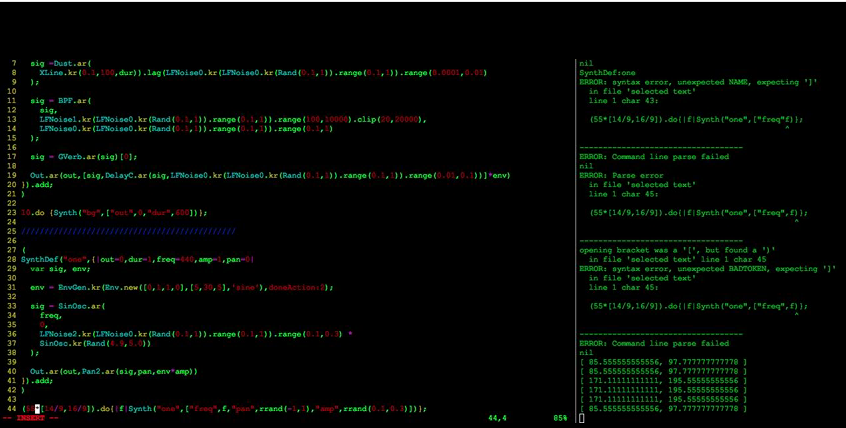
\includegraphics[scale=0.5]{./imagens/sc_drone.png}
%\caption{Improviso com \emph{drones} no SuperCollider \textbf{Fonte}: \url{https://www.youtube.com/watch?v=b8j4umQ2lIE}. }
%\label{sc_drone}
%\end{center}
%\end{figure}

%\subsection{Música eletrônica de Pista}\label{sec:musica_vanguarda_pista}

%Somado a todos esses elementos, existe a imagem já descrita de um DJ que se utiliza destas técnicas e estéticas para controlar seu \emph{set} (embora seja possível assumir que esta personagem pode utilizar outros dispositivos, como sintetizadores e baterias eletrônicas, todos eles presentes em um computador) e promover uma música na qual a dança é elemento central. É importante deixar claro que uma cultura DJ possui suas peculiaridades dependentes de contexto social: por exemplo, um dj europeu/norte-americano está em uma configuração social diversa do dj latino-americano e africano. Se até o momento temos discutido práticas musicais, na sua maioria, a partir de pessoas que falam o inglês como sua primeira língua, é natural supor que esta cultura DJ que falamos no \emph{livecoding} faz parte de uma cultura anglófona.

%Esse fenômeno de apropriação das MA, MG, MP e DJ, na cultura musical dos países rotulados como desenvolvidos, pode ser entendido a partir daquilo que Fernando  \citeonline{iazzetta_musica_2009} chamou de "sinergia de produções, que em sua diversidade compartilham dos mesmos elementos sociais e culturais" \cite[p.~152]{iazzetta_musica_2009}. Mais especificamente, trata-se de um fenômeno em sentido mais amplo das produções musicais usando o computador; mas buscarei encarar a questão no \emph{livecoding} da mesma maneira, como uma sinergia entre boates, casas noturnas e ambientes informais com ambientes de produção de conhecimento (universidades, escolas de música, faculdades de engenharia).

%Primeiro é necessário esclarecer se a apropriação foi intencional ou não.  O discurso do manifesto de \citeonline{ward_live_2004} indica uma consciência parcial dos autores a respeito desta sinergia. No entanto é discutível se esse cruzamento de gêneros é mais um reflexo das transformações sociais e culturais que o computador trouxe consigo do que algo intencional: o uso deliberado de muitas ferramentas de um estúdio portátil, a expansão de possibilidades de produção musical através das redes de computadores, a troca de informações a respeito do uso de novos \emph{softwares} entre músicos acadêmicos e não-acadêmicos , trouxe à tona diferentes comunidades daquela ou outra tecnologia. De forma semelhante, no \emph{livecoding}, as novas possibilidades tecnológicas em contato com modos de fazer música já estabelecidos possiblitaram a emancipação de novas práticas, o que por sua vez, capacitou o cruzamento de estéticas (tudo isso, no entanto, visto apenas pela ótica das culturas de pessoas que falam o inglês como primeira língua).

%Poderia ser questionado se o intercruzamento de gêneros musicais no \emph{livecoding} depende dos \emph{softwares}.  \citeauthoronline{iazzetta_musica_2009} responderia não, mas que dependem de uma articulação entre produções musicais e seus compositores, que carregam diferentes formações teóricas. Esse problema é colocada da seguinte forma:


%Embora seja possível considerar uma "comunidade Max/MSP", ela está dentro de uma população contendo as comunidades "SuperCollider", "PureData", "ChucK", indicando apenas alguns. 

%Dentro dessa população, surgem as pequenas comunidades de \emph{softwares} de \emph{live coding}, pela utilização e invenção de mini-linguagens pouco usadas, se comparadas com as do parágrafo acima. No contexto anglófono, essas pequenas comunidades apropriam um termo, segundo \citeonline{collins_algorave:_2014}, \emph{algorave}. 

 



